\chapter{Pipe}
\thispagestyle{empty}

Una pipe dal punto di vista del sistema operativo è un file gestito come una coda FIFO. 
Spesso esiste un processo produttore che deposita i dati in esso, e uno consumatore che li raccoglie.

\paragraph*{}
In \textit{POSIX} per creare una pipe si utilizza la funzione \textbf{int pipe(int fd[2])}, che accetta in ingresso due file descriptor, uno per la lettura ed uno per la scrittura.
Dopo averla creata l'utilizzo è analogo ai file, si usa \textbf{write(fd[1], ...)} e \textbf{read(fd[0], ...)}

Un alternativa prevede di usare \textbf{mknod}\footnote{mknod è abbastanza generico, prevede la creazione di altri tipi speciali di file, va usato il parametro \textit{p} per generare una pipe. Un alternativa è \textbf{mkfifo} che genera direttamente una pipe.}, che permette di aprire le pipe con una semplice \textit{open} e permette l'assegnazione di un nome identificativo.

\paragraph*{}
Spesso si utilizzano le pipe per la comunicazione padre-figlio tra processi, infatti il processo figlio eredita i file aperti, quindi le pipe. Generalmente la comunicazione è unidirezionale.

Un altro uso tipico lo si vede nei comandi shell quando si usa l'operatore \textbf{$\vert$}. Ciò che sta a destra prende in  input quello che esce da ciò che sta a sinistra. (e.g. \textit{cat documento.txt $\vert$ sort)}. La shell si occupa di generare il codice corretto che permette lo scambio delle informazioni.

\paragraph*{}
Un altro meccanismo che le shell usano per gestire l'input-output sono le \textbf{ridirezioni}. 

Se volessi ridirezionare l'output di un programma all'interno di un file userei \textbf{ps $>$ file.txt} \footnote{uso \textbf{$>>$} se voglio appendere al file senza sovrascriverlo.}. 

Se volessi invece ridirezionare lo standard error di un programma: \textbf{ps $2>$ file.txt}.

Allo stesso modo posso prendere rendere un file un input per un programma con: \textbf{sort $<$ file.txt}.

\begin{figure}[!ht]
    \begin{subfigure}{.5\textwidth}
    \centering
      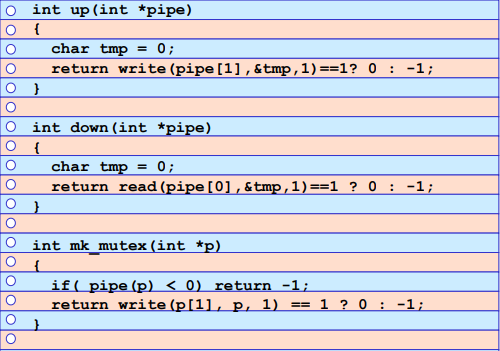
\includegraphics[width=1\linewidth]{assets/semaforoUno8.png}
    \end{subfigure}%
    \begin{subfigure}{.5\textwidth}
    \centering
      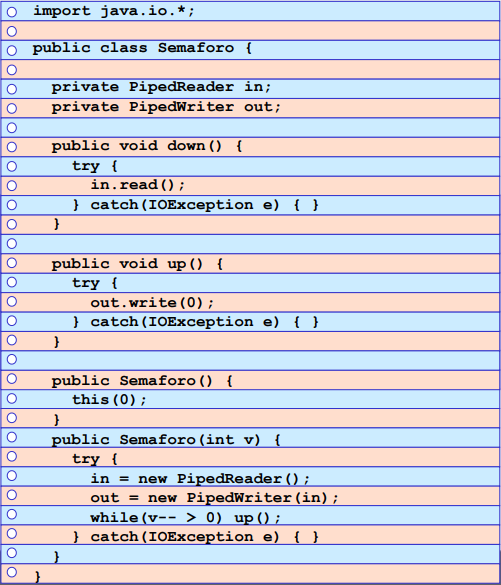
\includegraphics[width=0.9\linewidth]{assets/semaforoDue8.png}
    \end{subfigure}
    \caption{Realizzazione di un semaforo in C e Java tramite pipe.}
  \end{figure}

\paragraph*{}
In C esistono delle funzioni a più alto livello simili alle \textit{fopen} ma per le pipe: \textbf{popen} e \textbf{pclose}.

\paragraph*{}
Quando un processo padre condivide una pipe con il processo figlio spesso si utilizza l' \textbf{I/O bufferizzato}, ovvero un meccanismo di caching che riduce il numero di operazioni input/output: solo quando il buffer è pieno viene chiesto l'intervento del sistema operativo che scrive su disco le informazioni salvate sul buffer.


\paragraph*{}
\paragraph*{}
\begin{figure}[H]
    \centering
    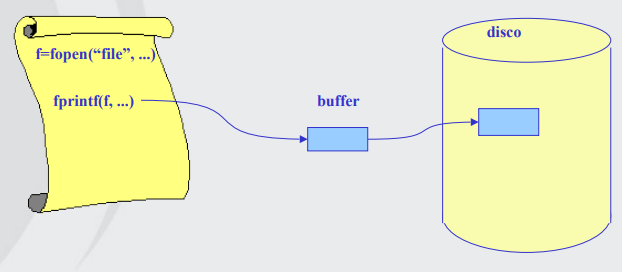
\includegraphics[width=0.6\linewidth]{assets/buffer8.png}
\end{figure}

\paragraph*{}
Allo stesso modo anche il sistema operativo usa una sua cache per ridurre le operazioni su disco. Con il comando \textbf{sync} si forza la scrittura.


\paragraph*{}
\paragraph*{}
\begin{figure}[H]
    \centering
    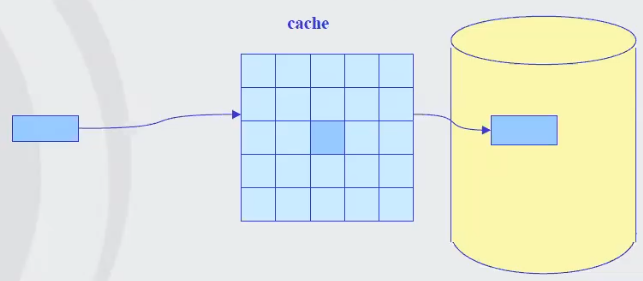
\includegraphics[width=0.6\linewidth]{assets/cache8.png}
\end{figure}
